\documentclass[a4paper,10pt]{article}
\usepackage[utf8]{inputenc}
\usepackage{graphicx}
\graphicspath{ {./graphs/} }
\graphicspath{ {./code/} }


\title{\textbf{Operating Systems ID1206} \\ 
\textbf{Seminar II Report}}

\author{Emil Ståhl}

\begin{document}

\maketitle
\textbf
{\\1. Introduction\\\\}
This report covers the implementation of dynamic memory allocation library functions written in C, more specific malloc( ) and free( ). In order to be able to distinguish the built-in versions of these functions this report will refer to its implementations as dalloc( ) and dfree( ). As described by the man pages, the malloc( ) function allocates size bytes on the heap and returns a pointer to the allocated memory. The free( ) function frees the memory space pointed to by the pointer, which must have been returned by a previous call to malloc( ). \\\\Dynamic memory allocation on the heap is needed when the amount of memory to be used is not known at compile time, or if it is obscenely large. Otherwise the memory could be allocated on the stack instead.  However,  in order to implement an efficient memory allocator there exist a number of hassles that need to be solved in order to get an allocator that uses memory as efficient as possible. The main topic covered in this work is to obtain a deeper understanding of the problems that dynamic memory allocation results in and how they can be solved to improve performance.

\maketitle
\textbf
{\\2. Main problems and solutions\\\\}
This section covers the different challenges that emerge when working with dynamic memory allocation. Firstly, a general description of the implementation is given.


\maketitle
\textbf
{\\2.1 Implementation of dalloc( ) and dfree( )\\\\}
In order to get up and running we need to create a new block of memory (arena), this is done using the mmap( ) UNIX system call that allocates a memory area that is as large as possible,  in this case it has been set to 64 KB. However, due to that mmap( ) is part of the kernel space it is a hugely slow operation to do. The dalloc( ) and dfree( ) library functions solve this problem since they run in user space. When the block has been created it is inserted into a ”free list” (flist) that will hold all free blocks of memory. Initially, the flist will consist of the whole arena block but will soon be split up into smaller blocks as the process allocates more memory using the dalloc( ) procedure.
\\\\Upon calling dalloc( ), the first thing that is done is adjusting the requested memory size so that it is bigger than 8 bytes as well as a multiple of 8. When the correct size is determined it is passed to the find( ) procedure that tries to find a block of the given size in the free list and if found it also checks if the chosen block can be split up. If the block is split the remaining part is inserted into the free list of blocks. If a block is found that is at least the size that was searched for it is returned to the dalloc( ) procedure. Back in dalloc( ) the block is then passed to the HIDE( ) procedure that hides the header. I.e returns a pointer to the beginning of the data segment.
\\\\In order to free a block previously allocated by dalloc( ) a pointer to the block is passed to the dfree( ) procedure. The first thing that is done is to include the head of the given block since the pointer points to the beginning of the data segment and not the actual incipience of the block. The block is then passed to the merge( ) procedure that checks if it is possible to merge the current block with its immediate neighbors. If, for example, the block before is free the two blocks are merged in the following manner: \\

\includegraphics[scale=0.35]{code/Merge.png}\\The merged block is then inserted in the beginning of the list with free blocks.

\maketitle
\textbf
{\\\\3. Possible improvements\\\\}
There are a number of ways to improve the performance of the implementation. One such amelioration is to do less work when searching for a new block in the free list. In the first implementation, every newly freed block is inserted at the beginning of the list of free blocks. This may result in that the algorithm needs to traverse the whole list looking for a suitable block as well as split it given that the block is big enough. The solution to this may be to keep the free list ordered with the smallest blocks at the beginning. \\\\By keeping the list ordered it is possible to find the block that best fit the requested size without needing to go thru the full list. The best fit is probably a block that does not need to be split, and thus resulting in less work when a block is searched for. \\\\To implement the desired behavior a new procedure orderInsert( ) is added. The procedure utilizes the insertion sort algorithm to determine where in the list a given block should be inserted in order to keep the list ordered.

\maketitle
\textbf
{\\\\\\\\4. Benchmarking\\\\}
For all benchmarking in this report, a benchmarking program written in C will be used. The program will take a buffer size, max size of request and a number of desired allocations. For all of the benchmarks, a buffer size of 100 blocks and a maximum size of 100 will be used. In addition to that, the benchmarking will perform a total of 1.000 memory allocation operations. However, when evaluating the free list length there will be several tests performed ranging from 1.000 - 10.000 allocations. \\\\The test program will enter a loop and at random choose either to allocate or free (granted there is something to free) memory every iteration. The probability to allocate memory is slightly higher than to free it, so that it can test the performance of high amounts of memory allocated. When there have been as many allocations of memory as specified by the arguments, the program terminates. While allocating memory, the program writes the current number of allocations as well as the time it took for the operation to complete (in milliseconds). \\\\There were two separate benchmarks performed for the two versions of the implementation (unordered and ordered free list). For the first test, the program writes the current number of allocations as well as the time it took for the allocation to complete (in milliseconds). The second test performs exactly the same operation but instead prints the length of the free list for every allocation completed. When all allocations have been completed, an average length of the free list is calculated. 

\begin{footnotesize}
\begin{center}{
\centering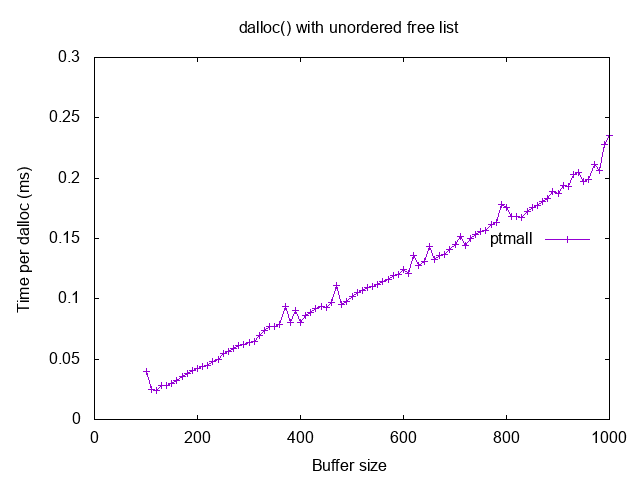
\includegraphics[scale=0.7]{graphs/ptmall-unordered.png}\par
\caption{Figure 4.1: The time required for 1.000 memory allocations with an unordered free list.}}
\end{center}
\end{footnotesize}


\begin{footnotesize}
\begin{center}{
\centering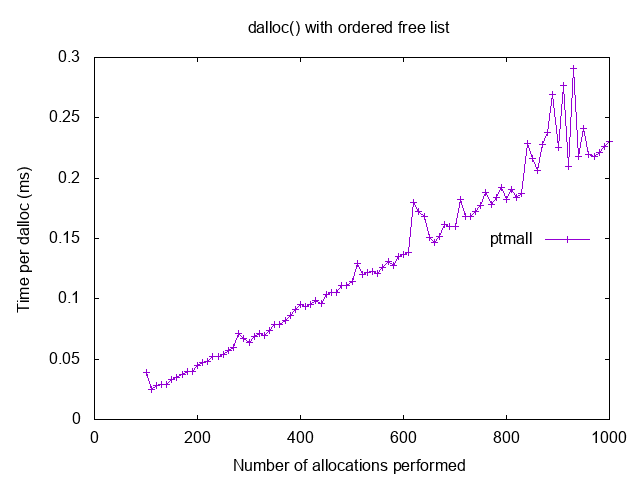
\includegraphics[scale=0.7]{graphs/ptmall-ordered.png}\par
\caption{Figure 4.2: The time required for 1.000 memory allocations with an ordered free list.}}
\end{center}
\end{footnotesize}

\begin{footnotesize}
\begin{center}{
\centering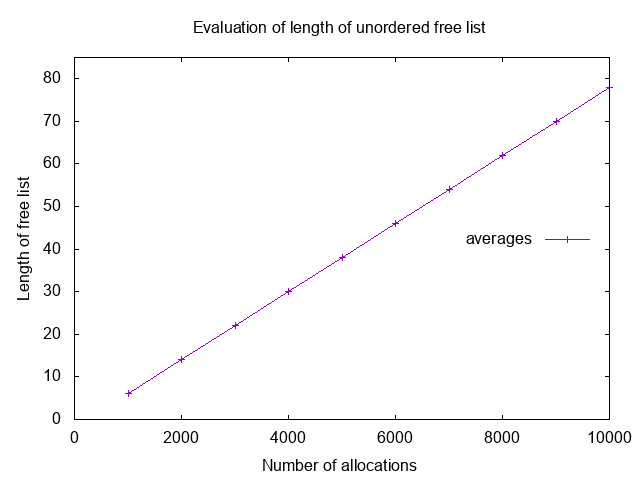
\includegraphics[scale=0.7]{graphs/averages-with-unordered.png}\par
\caption{Figure 4.3: The length of the free list with regards to the number of allocations performed with an unordered free list.}}
\end{center}
\end{footnotesize}

\begin{footnotesize}
\begin{center}{
\centering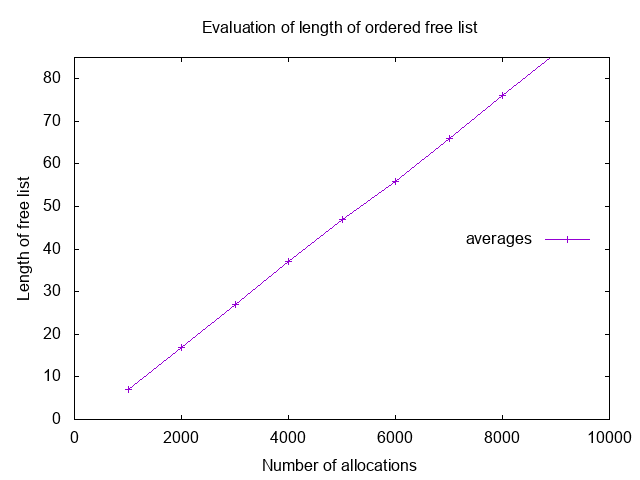
\includegraphics[scale=0.7]{graphs/averages-with-ordered.png}\par
\caption{Figure 4.4: The length of the free list with regards to the number of allocations performed with an ordered free list.}}
\end{center}
\end{footnotesize}

\maketitle
\textbf
{\\5. Evaluation\\\\}
The evaluation of these results is that it seems to be that the first implementation with an unordered free list performs better than the one with an ordered list. The average time to allocate memory with an unordered list was 0,1112527473 ms as compared to the ordered implementation which on average took 0,1243406593 ms to complete. Similar results are shown when examining the length of the free list. The unordered list has on average a length of 6 to 78 blocks when performing 1.000 - 10.000 allocations. When working with the ordered list these numbers stretches from 7 to 96 blocks tested with the same number of allocations. The decrease in performance as well as increase of free list length is most likely a consequence of external fragmentation, i.e. too many small blocks are created which cannot be utilized. In addition to this, it takes time to order the free list every time a block is freed and inserted which decreases the performance even more. 

\maketitle
\textbf
{\\\\6. Optimizations\\\\}
There are several further optimizations that can be made to the implementation. One such could be to keep more lists of free blocks, for example one list for every multiple of 8 (16, 24, 32…128) and then one extra for everything else. Then it would require less searching when a new block is requested as well as it would be easier to sort each list. One could also experiment with other data structures. Maybe a tree structure of all the free blocks would work better?  

\maketitle
\textbf
{\\\\7. Conclusions\\\\}
This work has focused on implementing the memory allocation library functions dalloc( ) and dfree( ). Two different implementations were covered, one with an unordered list of free blocks and one where the list was sorted. Two different benchmarks were performed on each implementations which show that the best performing version was the one with the unordered list. This is probably due to external fragmentation as well as the extra work it takes in order to sort the list. However, there exists several optimizations that can be evaluated in future work. 

\end{document}
